\documentclass{article}

% Numbered, compressed citations (e.g. [3, 5-7]) -- matches NeurIPS house style.
\PassOptionsToPackage{numbers, compress}{natbib}

% Workshop submission (double-blind). For the camera-ready add ", final".
% NOTE: NeurIPS 2026 style not yet released; using the near-identical 2025 style.
\usepackage[dblblindworkshop]{neurips_2025}

\usepackage[utf8]{inputenc}
\usepackage[T1]{fontenc}
\usepackage{hyperref}
\usepackage{url}
\usepackage{booktabs}
\usepackage{amsfonts}
\usepackage{amsmath}
\usepackage{nicefrac}
\usepackage{microtype}
\usepackage{graphicx}
\usepackage{subcaption}

% =====================================================================
% VERSION 2 -- Full paper (compact build, < 8 pages).
% Framing: artifact-first, cloth-centered (per mentor). Related Work is
% folded into the citation-dense Introduction. Voice per CLAUDE.md; no
% em-dashes. Every number traces to docs/results-summary.md and
% docs/handoff-ablation.md; figures from make_figures.py.
% Citations: the 23-entry references.bib (13 provided + 10 web-verified).
% =====================================================================

\title{A Cloth Simulator That Knows When to Trust Itself:\\
Detector-Gated Hybrid Neural--Physics Rollouts}

\author{%
  Anonymous Author(s)\\
  Affiliation\\
  \texttt{email}
}

\begin{document}

\maketitle

\begin{abstract}
Cloth shows up everywhere in games and film, and lately in virtual try-on and
robot manipulation too. The catch is speed. The high-fidelity solvers people
trust, the Material Point Method (MPM) among them, inch forward in many tiny
sub-steps to stay stable, which rules them out for anything interactive. Learned
emulators flip that trade-off: they are fast, but they pile up errors over a
long rollout, with nothing in the loop keeping the result physically honest. Classical solvers are accurate, but cost too much to
lean on every frame. We take a middle path. A fast graph-network emulator does the
ordinary work, and a cheap, interpretable deformation signal watches for the
frames where it is likely to slip (the folds, the fast contacts) and routes just
those to an implicit mass--spring fallback. What we did not expect is that the
hand-off matters more than the detector. Switching between two solvers that are
each perfectly stable on their own can land you worse off than either alone, and
the fix is surprisingly simple: once the fallback engages, make it stay put for a
while. On held-out cloth the hybrid runs $1.8$--$2.0\times$ faster than full
physics, trims the emulator's positional drift by $30.8\%$, and the detector flags
hard frames at $0.98$ AUROC. We also report the tidy fixes that looked obvious and
did not work.
\end{abstract}

\section{Introduction}

Picture a character's skirt drifted by the wind, or a flag snapping on a pole.
Rendering such \emph{cloth} on screen almost always means simulating the
physics: springs and masses in the classic setup~\citep{baraff1998}, or a
continuum discretized onto a background grid, which is what the Material Point
Method does~\citep{jiang2016mpm, hu2018mlsmpm, stomakhin2013snow}. Cloth then
drove the method in its own directions. Thin-shell formulations, anisotropy along
warp and weft, contact and self-contact resolved right on the particle--grid
transfer~\citep{guo2018thinshells, wolper2020anisompm}, all of it layered on top of
the collision machinery cloth has always needed~\citep{bridson2002collisions}. While it works, it is not cheap. Explicit schemes require tiny time steps or they blow up.
Implicit ones trade that for large linear solves. Either way, a single frame is many
sub-steps, and the cost climbs quickly as you refine the mesh to catch fine
wrinkles~\citep{zhang2025clothres}. For an offline render, this works just fine. For something you
want to interact with and watch respond, it falters. That is what sends people searching for a
cheaper stand-in that still moves like fabric.

The obvious stand-in is a network that has watched enough simulation to imitate it.
Graph networks are the default choice. They learn particle dynamics by message
passing~\citep{sanchez2020gns}, and MeshGraphNets does the mesh-based version, which already covers cloth~\citep{pfaff2021mgn}; both rest on the
broader graph-network framework~\citep{battaglia2018gn}. Related particle methods
learn deformable and fluid dynamics directly~\citep{li2019dpi, ummenhofer2020cconv}.
Cloth has a specialized branch of its own: the networks that predict garment drape
and dynamics from body pose, sometimes with physics folded into the architecture or
the loss~\citep{zhao2024physcloth, bertiche2021pbns, santesteban2022snug,
grigorev2023hood}. A different approach keeps the numerical solver and learns only a
correction to it~\citep{um2020solver}, which differentiable simulators make
practical by exposing gradients straight through the solver~\citep{hu2020difftaichi}.
These are all genuinely fast. The problem surfaces over time: a pure-neural rollout
feeds its own output back in, so a small slip this step becomes the input to the
next, and the trajectory drifts, with nothing holding it to the
physics~\citep{sanchez2020gns}. The natural remedy is running the emulator most of the time and dropping
back to a real solver on the hard frames, and we are not
the first to reach for it; the closest precedent runs a neural MPM for fluids with a
classical solver as a safety net~\citep{xu2025hybridmpm}, and that is precisely the
design we carry over to cloth. Where we change the approach is crucial. That work, and
hybrids like it, mostly ask how accurately you can \emph{spot} the hard frames;
they don't consider what happens at the seam, when one solver hands control to the
other. The seam, it turns out, is the highlight of the story.

Three pieces make up the system. An MLS-MPM cloth solver~\citep{hu2018mlsmpm,
jiang2016mpm} is the reference, generating the training data and defining what
``correct'' even means here. The emulator is a MeshGraphNets-style graph
network~\citep{pfaff2021mgn} trained on short rollouts of its own predictions. It uses the
pushforward trick from the PDE-solver literature~\citep{brandstetter2022mpnn} and a
method closely related to the training noise used in GNS~\citep{sanchez2020gns}. The fallback mechanism is
a plain implicit mass--spring step~\citep{baraff1998}, inspired by the seed
hybrid's classical safeguard~\citep{xu2025hybridmpm}. A lightweight detector, which monitors the frame-to-frame change in a local strain estimate, determines when this fallback is triggered.
One point is worth stating outright, as it colors how the entire system should be evaluated: the fallback is not the ground truth. It is a low-fidelity model in its own right, meaning the hybrid approach stitches together two different approximations, neither of which is the reference. How long the fallback remains active and how often control changes hands, is where quality is won or lost, far more than in the detector that trips it. We also tried the standard fixes you would typically reach for first: fine-tuning the
emulator on the fallback's states in a DAgger-style
loop~\citep{ross2011dagger}, and blending the two solvers across the switch rather
than applying a hard cut. Neither approach helped, and explaining why they did not succeed is part of what we are reporting. For speed, inference runs in fp16~\citep{micikevicius2018mixed}, which we
find essentially lossless in this case.

\paragraph{Contributions.} 
There are three concrete contributions:
\begin{itemize}
  \item \textbf{A fast, faithful hybrid cloth simulator.} We introduce a graph-network emulator backed by a low-fidelity implicit fallback that activates only when triggered by an interpretable deformation signal. This approach is $1.8$--$2.0\times$ faster than the reference MPM, shows 
  $30.8\%$ less positional drift on a held-out drape, and achieves a detector score of $0.98$ AUROC.
  \item \textbf{The hand-off, not the detector, governs the rollout.} Naive switching can perform worse than using either solver alone; we found that a minimum-dwell (hysteresis) rule provides the most dependable solution. Alternative approaches, such as DAgger-style fine-tuning and cross-solver blending, fail because the emulator and the fallback occupy different dynamics manifolds.
  \item \textbf{An honest account.} We provide a working GPU implementation with the speed-accuracy trade-off measured end-to-end, alongside a candid record of the approaches that did not work rather than setting them aside.
\end{itemize}

\section{Method}

\paragraph{Reference and data.} The reference is a Taichi MLS-MPM thin-shell cloth
solver~\citep{hu2018mlsmpm, hu2020difftaichi} configured on a $64\times64$ sheet
($4{,}096$ particles). We utilized two scenarios: \emph{drape} (where the sheet falls and settles without
pins) and \emph{collision} (where the sheet is pinned at two corners and drapes over a moving sphere).
Wind effects were deferred, as they were not stable enough at full resolution to be trusted for training data. We trained the model on a balanced dataset of $3{,}000$ clips ($1{,}500$ per scenario), with each clip storing per-frame positions, velocities, and accelerations.

\paragraph{Neural emulator.} We use a MeshGraphNets-style graph
network~\citep{pfaff2021mgn}: $L{=}5$ message-passing steps, hidden width $128$,
about $847$k parameters. The nodes carry the particle state and the edges follow the mesh.
The network maps $(x, v)$ to per-particle acceleration, which is then advanced using a semi-implicit Euler step. We removed the deformation gradient $F$ from the input because it is codimensional for a thin shell and its determinant drifts, which negatively impacted performance. Training
uses the pushforward curriculum~\citep{brandstetter2022mpnn}, which unrolls $K$ steps on the
model's own predictions and backpropagates through the integration, ramping
$K \to 5$. On a practical note, the naive unroll holds the
autograd graph for the whole batch and runs out of memory by $K{=}2$. Taking the backward pass per clip reduces
peak memory from $B{\times}K$ to $1{\times}K$ and makes the curriculum feasible.

\paragraph{Detector and routing.} We want a per-frame signal for \emph{where the
emulator will drift}, using only what a deployed no-$F$ rollout actually has:
positions. Ours is a position-based strain proxy, a local deformation gradient fit
by least squares from a particle's neighbourhood, tracked by its frame-to-frame rate
of change. It is deliberately \emph{not} the cosine-of-acceleration signal prior
hybrids default to, which targets locally hard dynamics like contact that our
emulator already handles. The rollout runs the emulator by default and, when the
proxy crosses a threshold, substitutes a fallback step. The subtlety is when to hand
back: a per-frame switch churns control, and that churn is what hurts (Sec.~\ref{sec:hybrid}),
so we add \emph{hysteresis}, staying in fallback until the signal drops well below
the trigger. This keeps control in one solver for a contiguous stretch; a
minimum-burst variant (stay $\ge K$ frames) behaves identically and makes the
mechanism plain.

\paragraph{Physics fallback.} An implicit mass--spring Euler step on the same
particles treated as mesh nodes~\citep{baraff1998}. Our initial CPU solver (using modified
preconditioned conjugate gradient) was correct but slow ($119$\,ms/frame). To improve performance, we developed a matrix-free GPU rewrite that forms no explicit system matrix and runs a fixed-iteration conjugate gradient solver under \texttt{torch.compile}. This optimization reduced the compute time to $3.55$\,ms, which is faster than the
MPM reference.

\section{Experiments}

\paragraph{Protocol.} Accuracy is measured using fp32 on held-out clips. Speed is evaluated on an A10G GPU with warmup and device synchronization. For the hybrid model, we tune the knobs (threshold,
hysteresis exit ratio) on one split and report results on a \emph{disjoint} split to ensure the metrics are independent of the tuning set. Positional error is calculated as per-particle L2
against the MLS-MPM reference. The detector is scored by AUROC against
$y_t = \mathbf{1}[\,\text{L2}(t) > 0.10\,\text{m}\,]$.

\paragraph{Surrogate accuracy.} Table~\ref{tab:rq1} shows the emulator's performance. 
The results split by scenario, contrary to our initial expectations. On \emph{collision} scenario, the case
we worried about most, the emulator tracks tightly and nearly conserves energy (drift $0.017$).
On the \emph{drape} scenario, it stays stable but the swing slides out of phase late in a long rollout. As a result, the final L2 and energy numbers reflect phase mismatch rather than a blow-up.
This asymmetry is exactly what the detector and fallback mechanisms are designed to cover.

\paragraph{Detector.} The position-only strain proxy separates drift frames at
$0.980$ (for drape) and $0.985$ AUROC (for collision). This matches the $F$-based signal but
is computable from predicted positions, meaning it survives deployment (Fig.~\ref{fig:detector}).
Conversely, the cosine-of-acceleration signal that prior hybrids use scores $0.65$ on drape, which is the
wrong target. One trap worth flagging: a classifier on all features \emph{pooled}
across scenarios scores well by quietly guessing the scenario while performing worse
within each. Therefore we report per-scenario, where ``strain proxy plus threshold'' serves as the
detector.

\paragraph{Speed.} Table~\ref{tab:speed} has the performance numbers from our latest benchmarks. Initially, the fp32 net ($9.9$\,ms) is actually \emph{slower} than well-tuned Taichi
MPM ($5.6$\,ms), and the CPU fallback was significantly slower at ($119$\,ms). However, this was an implementation issue rather than a conceptual one. By using fp16 with \texttt{torch.compile} the network execution time dropped to
$2.1$\,ms (lossless per step, $0.07\%$ acceleration error), and the matrix-free GPU
fallback to $3.55$\,ms. End-to-end in the rollout loop, the hybrid approach is
$1.8$--$2.0\times$ faster than the full MPM. While this is lower than our initial target of $3$--$5\times$ it represents a real, end-to-end measured speedup.

\begin{table}[t]
  \centering
  \begin{minipage}[t]{0.46\linewidth}
    \centering
    \caption{Neural emulator alone, held-out ($400$-step rollouts). Collision is the
    strong case; drape drifts out of phase late.}
    \label{tab:rq1}
    \small
    \begin{tabular}{lcc}
      \toprule
      metric & drape & collision \\
      \midrule
      one-step accel.\ err. & \multicolumn{2}{c}{$0.405$ m/s$^2$} \\
      L2 @ $200$ (m)        & $0.017$ & $0.005$ \\
      L2 final (m)          & $0.19$  & $0.077$ \\
      energy drift          & $0.70$  & $\mathbf{0.017}$ \\
      \bottomrule
    \end{tabular}
  \end{minipage}\hfill
  \begin{minipage}[t]{0.5\linewidth}
    \centering
    \caption{Held-out drape, hysteresis tuned on $17$ clips, reported on $18$
    disjoint clips. Hybrid matches pure-fallback accuracy on about half the physics.}
    \label{tab:hybrid}
    \small
    \begin{tabular}{lcc}
      \toprule
      policy & L2 final (m) & vs.\ neural \\
      \midrule
      neural                        & $0.186$ & n/a \\
      fallback-only                 & $0.128$ & $+31.3\%$ \\
      \textbf{hybrid (hyst.)}       & $\mathbf{0.129}$ & $\mathbf{+30.8\%}$ \\
      \bottomrule
    \end{tabular}
  \end{minipage}
\end{table}

\begin{table}[t]
  \centering
  \caption{Per-frame wall-clock, $4{,}096$ particles, A10G. Fair basis: neural is one
  forward step ($\mathrm{dt}{=}10^{-3}$); MPM is $10$ sub-steps ($\mathrm{dt}{=}10^{-4}$)
  for the same physical time; fallback is one stable step.}
  \label{tab:speed}
  \small
  \begin{tabular}{lccccc}
    \toprule
    & full-MPM & neural fp32 & neural fp16+compile & fallback CPU & fallback GPU \\
    \midrule
    per-frame     & $5.6$\,ms & $9.9$\,ms & $2.1$\,ms & $119$\,ms & $3.55$\,ms \\
    vs.\ full-MPM & $1.0\times$ & $0.6\times$ & $2.65\times$ & n/a & n/a \\
    \bottomrule
  \end{tabular}
  \\[2pt]
  \footnotesize Hybrid, end-to-end in the rollout loop: $\mathbf{1.8\text{--}2.0\times}$ faster than full-MPM.
\end{table}

\paragraph{Hybrid accuracy, and the hand-off.}
\label{sec:hybrid}
Here is the interesting finding regarding the solvers. Each solver alone performs well on drape (pure neural ends at L2
$0.190$, pure fallback at $0.124$). However, switching every frame the raw detector fires results in an L2 of $0.389$, worse than \emph{both} individual approaches. The solvers are individually stable; the
switching is what causes the performance to drop. Each switch hands one solver a state produced by the other, which is off its own manifold, causing the mismatch to compound. Figure~\ref{fig:decay}
measures this effect: immediately after a switch the two solvers' accelerations, evaluated on the
same state, disagree $1.5$--$2.7\times$ more than in steady state, relaxing over
about $10$ frames. Every hand-off injects a $\sim$$10$-frame transient; constant switching means paying this penalty continuously. This insight reframes our approach. At a \emph{matched}
fallback budget, error falls monotonically as switches drop (Fig.~\ref{fig:switches}).
Naive routing requires $\sim$$22$ switches to reach an L2 of $0.185$, while sticky hysteresis needs
$\sim$$5$ switches to reach $0.124$, a third lower on the \emph{same} physics.
Figure~\ref{fig:time} shows the same policies over time, which remain identical until the fallback
first fires (around step $200$), then fanning out by how much they churn. When the
hysteresis is tuned on a disjoint split, the hybrid model holds up well on unseen clips
(Table~\ref{tab:hybrid}): It achieves $+30.8\%$ over pure neural approach at a $49\%$ fallback rate, statistically
matching accuracy of pure-fallback approach at half of its physics cost. On collision, the detector
fires on $0\%$ of frames, correctly, since the emulator there ($0.033$) already outperforms
the fallback ($0.28$), so the hybrid quietly reduces to the emulator.

\begin{figure}[t]
  \centering
  \begin{subfigure}{0.33\linewidth}
    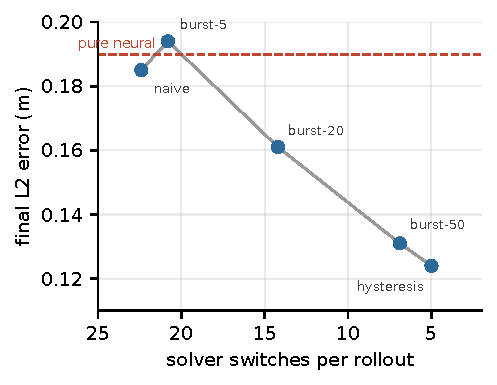
\includegraphics[width=\linewidth]{figures/fig_switches_vs_error.pdf}
    \caption{}\label{fig:switches}
  \end{subfigure}\hfill
  \begin{subfigure}{0.33\linewidth}
    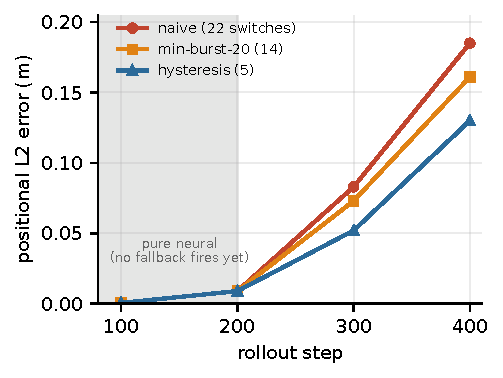
\includegraphics[width=\linewidth]{figures/fig_error_over_time.pdf}
    \caption{}\label{fig:time}
  \end{subfigure}\hfill
  \begin{subfigure}{0.33\linewidth}
    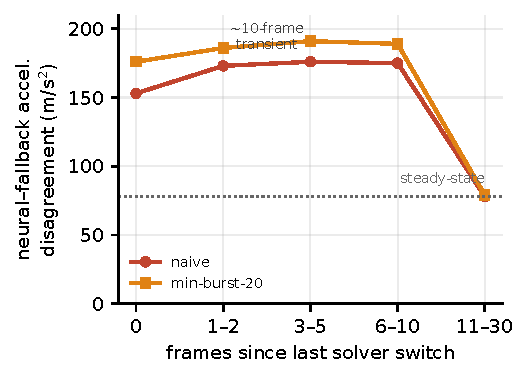
\includegraphics[width=\linewidth]{figures/fig_disagreement_decay.pdf}
    \caption{}\label{fig:decay}
  \end{subfigure}
  \caption{The hand-off, not the detector, governs the rollout.
  \textbf{(a)} At a matched fallback budget, final error falls monotonically as
  switches drop; sticky routing beats fragmented routing on the \emph{same} physics.
  \textbf{(b)} The policies are identical until the fallback first fires
  ($\sim$step $200$), then separate by how much they churn.
  \textbf{(c)} The mechanism: after each switch the two solvers disagree well above
  their steady-state level for $\sim$$10$ frames, a transient that fragmented
  switching re-triggers constantly.}
  \label{fig:handoff}
\end{figure}

\begin{figure}[t]
  \centering
  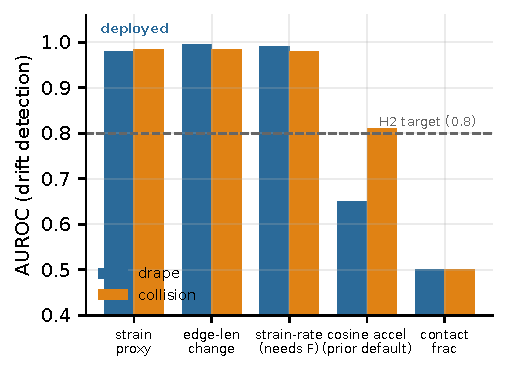
\includegraphics[width=0.55\linewidth]{figures/fig_detector_auroc.pdf}
  \caption{Detector separability (AUROC) by feature and scenario. The deployable
  position-based strain proxy matches the $F$-based signal and clears the H2 target;
  the cosine-of-acceleration signal used by prior hybrids does not.}
  \label{fig:detector}
\end{figure}

\paragraph{What did not work.} Two natural attempts to \emph{remove} the per-hand-off
cost, ultimately failed for the same reason. They are worth noting because they are the first
solutions a reader will consider. \emph{DAgger fine-tuning}~\citep{ross2011dagger}: Training the emulator on states visited by the fallback mechanism fails to resolve the issue. Querying the MPM reference at these states is unstable because they lie off the MPM manifold, resulting in one-step accelerations of $250$--$1600$\,m/s$^2$ compared to a physical limit of $10$--$30$\,m/s$^2$.
Alternatively, using the fallback's \emph{own} accelerations introduces a distributional incompatibility with
the MPM data, causing the normalized loss to explode. \emph{Blending}: Crossfading the two next-states rather than executing a hard cut yields \emph{worse} results at a matched budget. A convex blend of states from different manifolds lands off both, which prolongs off-manifold exposure. Ultimately, both failures demonstrate a structural gap between two distinct dynamics. The solution is to cross this gap less frequently rather than attempting to smooth the crossing.


\section{Limitations and Conclusion}
Here are a few caveats regarding the current results: The speedup is $\sim$$2\times$, rather than the $3$--$5\times$
we first targeted. Results cover drape and collision at a $64\times64$ resolution. Wind has been deferred, and larger resolutions have been timed but not accuracy-validated. The accuracy gain
\emph{needs} hysteresis, so it is a property of the schedule rather than an inherent benefit. ``Matches
physics'' indicates alignment with the low-fidelity mass--spring \emph{fallback}, and not the exact MPM
reference. A single scenario-agnostic detector remains future work.

Those aside, the artifact stands: a graph-network cloth emulator with an
interpretable, position-only drift detector and a cheap implicit fallback that runs
$1.8$--$2.0\times$ faster than full MPM while cutting drift by $30.8\%$ on held-out
cloth. The transferable lesson is the one we did not anticipate. When you couple a
neural emulator to a physics solver, the hand-off between them is a first-class design
variable. Switching too often can cause two good solvers to make a bad rollout. The reliable
fix is not a cleverer blend or more fine-tuning (both of which failed) but simply
switching less. For anyone building a simulator meant to know when to trust itself,
that is the part worth remembering.

\bibliographystyle{plainnat}
\bibliography{references}

\end{document}
